% !TEX encoding = UTF-8 Unicode
\RequirePackage{fix-cm}
\documentclass[a4paper,10pt,UTF8]{paper}
%\documentclass[a4paper,10pt,UTF8]{ctexart}

\usepackage[english]{babel}
\usepackage{fancyhdr,array,lastpage,amsmath,mathtools,enumitem,graphicx,multirow,tocbibind,longtable,makecell,varwidth,titlesec,bm,booktabs,comment,minted}
\usepackage{enumitem}
\usepackage{hyperref}
\hypersetup{hidelinks}




\usepackage[left=2.54cm,right=2.54cm,top=2.54cm,bottom=2.54cm]{geometry}
\usepackage[font=footnotesize,labelfont=bf]{caption}
\usepackage{tikz,flowchart}
\usepackage{ctex}
\usepackage{xeCJK}%中文字体
\usetikzlibrary{shapes,shapes.geometric,arrows,matrix,calc}
\usetikzlibrary{circuits.logic}

% \usetikzlibrary{circuits.logic.custom}
\usetikzlibrary{circuits.logic.IEC}
\usetikzlibrary{shadows}
\usepackage{listings}
\usepackage[Q=yes]{examplep}
\usepackage{fancyhdr}
\usepackage{alphalph}
\usepackage{indentfirst}

% \setCJKsansfont{黑体}
\setmainfont{PingFang SC}
\setCJKmainfont{PingFang SC}
\setCJKsansfont{PingFang SC}
\setmonofont{Monaco}

\newenvironment{sol}
  {\par\vspace{2mm}\noindent{\bf Solution}. }

\lstset{escapeinside=``, breaklines=true, frame=none, extendedchars=false, basicstyle=\ttfamily, showstringspaces=false}


\setlength{\parindent}{2em}
\setlength{\parskip}{1.5ex plus 0.5ex minus 0.2ex}
\linespread{1.1}

\bibliographystyle{plain}

\numberwithin{equation}{section}
\numberwithin{figure}{section}


\setcounter{secnumdepth}{3}
\setcounter{tocdepth}{3}

\title{华东师范大学计算机科学技术系上机实验报告}

\begin{document}
\pagestyle{fancy}
\chead{\small\color{gray}华东师范大学计算机科学技术系上机实验报告}
\lhead{}
\rhead{}
\makeatletter
\def\headrule{{\if@fancyplain\let\headrulewidth\plainheadrulewidth\fi%
    \color{gray}\hrule\@height 0.2pt\@width\headwidth}
    \vspace{6mm}}
\makeatother

\newcommand{\HRule}{\rule{\linewidth}{1mm}}
\newcommand{\dai}{\textbf{Dais-CMX16$^+$}}

{\center {\huge \bfseries \LARGE{华东师范大学计算机科学技术系上机实验报告}} \\ [0.8cm]
    
    \small{
        \begin{minipage}[t]{.32\linewidth}
            \textbf{课程名称:}嵌入式原理与实践\\
            \textbf{指导教师:}沈建华\\
            \textbf{上机实践名称:} 模数转换器\\
            \textbf{实践编号:}实验 11
        \end{minipage}
        \begin{minipage}[t]{.32\linewidth}
            \textbf{年级:}17 级\\
            \textbf{姓名:}朱桐\\
            \textbf{学号:}10175102111\\
            \textbf{组号:}A
        \end{minipage} 
        \begin{minipage}[t]{.32\linewidth}
            \textbf{上机实践成绩:} \\
            \textbf{创新实践成绩:} \\
            \textbf{上机实践日期:}2019/12/17\\
            \textbf{上机实践时间:}2 学时\\
        \end{minipage}
    }
    \HRule \\[0.5cm]
}

\definecolor{bg}{rgb}{0.95,0.95,0.95}
\newminted{asm}{bgcolor=bg}
\newminted{c}{bgcolor=bg}

\NewDocumentCommand{\cw}{v}{\texttt{\textcolor{black}{#1}}}

\section{实验目的}

\begin{enumerate}
    \item 了解ADC工作过程
    \item 掌握MSP432 ADC单通道的配置和中断的使用
    \item 进一步熟练UART的配置和使用
\end{enumerate}

\section{实验设备}

\begin{enumerate}
    \item 软件Keil5
    \item MSP-EXP432P401R LaunchPad开发板
    \item 电位器模块
\end{enumerate}


\section{实验内容}

\begin{enumerate}
    \item 掌握MSP432 ADC单通道配置和中断;
    \item 熟练MSP432 UART配置和使用;
    \item 完成课堂练习:旋钮台灯的实现;
\end{enumerate}

\section{实验原理}

\subsection{ADC 简介}

ADC,Analog-to-Digital Converter的缩写,指模数转换器,可将连续变化的模拟信号转换为离散的数字信号。真实世界的模拟信号,例如温度、压力、声音或者图像等,需要转换成更容易储存、处理和发射的数字形式。模数转换器可以实现这个功能,在各种不同的产品中都可以找到它的身影。

\begin{figure}[h]
    \centering
    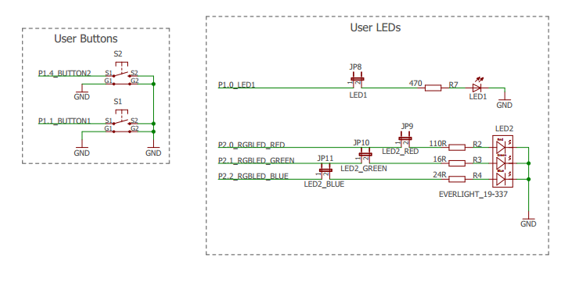
\includegraphics[width=0.9\textwidth]{img/1.PNG}
    \caption{相关原理图}
    \label{fig:1}
\end{figure}

SP432 包含一个 14 位的 ADC14 模块,支持快速 14 位模数转换。 ADC14 模块采用的是 SAR(逐次逼近)内核,有 32 个独立的缓冲区和对应的控制寄存器, 32 路单端/差分可选的外部输入通道。在最高分辨率时,最高转换速率可达 1Msps。

\begin{figure}[h]
    \centering
    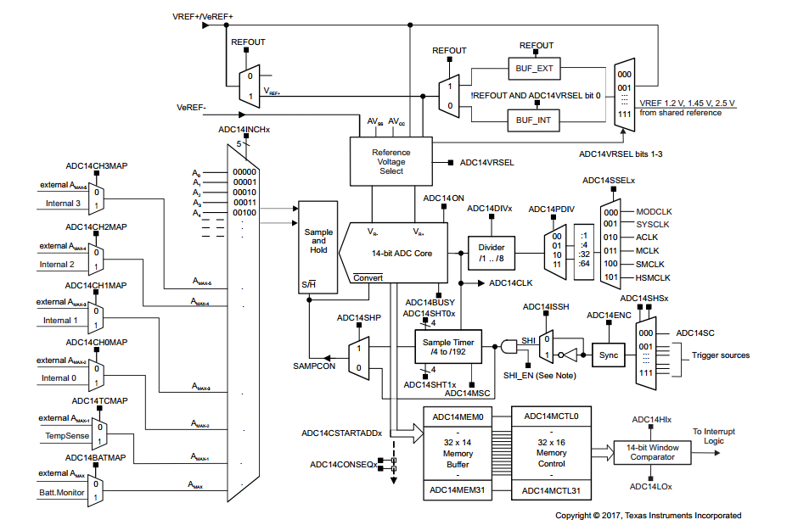
\includegraphics[width=0.9\textwidth]{img/2.PNG}
    \caption{数据通路}
    \label{fig:2}
\end{figure}



\subsection{实验所需函数}

\begin{ccode}
    void ADC14_enableModule  (void)
    
\end{ccode}

\begin{itemize}
    \item 功能描述:使能ADC 模块
\end{itemize}

\begin{ccode}
    bool ADC14_initModule (uint32_t clockSource, 
    uint32_t clockPredivider, uint32_t clockDivider,
    uint32_t internalChannelMask)  
\end{ccode}

\begin{itemize}
    \item 功能描述:初始化ADC 模块并设置时钟,同时配置内部/外部信号映射
    \item 参数描述 \\ clockSource    选择ADC 模块的时钟源 \\
          clockPredivider  时钟预分频 \\
          clockDivider      在预分频的基础上进行再一次的时钟分频 \\
          internalChannelMask     配置内部/外部引脚映射 \\
          
\end{itemize}


\begin{ccode}
    bool ADC14_configureSingleSampleMode (uint32_t
    memoryDestination, bool repeatMode)            
    
\end{ccode}

\begin{itemize}
    \item 功能描述:将ADC 模块配置为单通道采样模式
          
    \item 参数描述 \\ memoryDestination     选择存放转换结果的存储器 \\ repeatMode                选择是否反复进行采样转换
    \item   返回值: 若配置成功则返回True,否则返回False
\end{itemize}

\begin{ccode}
    bool ADC14_configureConversionMemory 
    (uint32_t memorySelect, uint32_t refSelect,
    uint32_t channelSelect, bool differntialMode)         
\end{ccode}

\begin{itemize}
    \item 功能描述:配置存放转换结果的存储器
          
    \item 参数描述 \\ memorySelect    选择要配置的存储器地址 \\
          refSelect            选择参考电压 \\ 
          channelSelect     选择ADC 采样通道 \\ differntialMode   选择是否使用差分模式采样
    \item   返回值: 若配置成功则返回True,否则返回False
\end{itemize}

\begin{ccode}
    bool ADC14_enableSampleTimer (uint32_t multiSampleConvert)      
            
\end{ccode}

\begin{itemize}
    \item 功能描述:使能采样定时器并配置反复采样/转换模式  
          
    \item 参数描述 \\ multiSampleConvert     选择采样/转换模式,可配置为手动或自动,手动模式下,每次ADC 转换结束需手动给出信号才进行下一次的采样/转换  
          
    \item   返回值: 若配置成功则返回True,否则返回False
\end{itemize}

\begin{ccode}
    void ADC14_enableConversion (void)    
\end{ccode}

\begin{itemize}
    \item 功能描述:使能ADC 转换值: 若配置成功则返回True,否则返回False
\end{itemize}

\begin{itemize}
    \item 功能描述: 使能UART模块指定中断
    \item 参数描述:moduleInstance  指定使用的UART模块
    \item mask      指定中断类型
\end{itemize}

\section{实验步骤}

\subsection{ADC 实验}

\begin{enumerate}
    \item 打开位于工程11\_01的adc工程;
    \item 点击编译并下载至LaunchPad开发板;
    \item 使用串口工具打开LaunchPad开发板XDS110 Class Application/User UART串口,串口配置参数:波特率为9600,8位数据位,无校验位,1位停止位,无流控;
    \item 将电位器杜邦线连接至开发板:黄线(OUT引脚)→开发板P5.5、红线(VCC引脚)→开发板3V3、黑线(GND脚)→开发板GND;
    \item 拧动电位器,观察串口工具中的回显数值,在实验报告中描述该实验现象,并简单说明其原因。
\end{enumerate}

打开串口工具,配置 URAT 端口后接受信息,发现得到的电压值在 $[0,3.3V]$ 之间。这符合我们的预期,因为我们把 VCC 接在开发板的 3.3V 电源上面

\subsection{课堂练习}

\begin{enumerate}
    \item 新建旋钮台灯keil工程,工程名为:light\_学号,并保存到工程11\_02文件夹;
    \item 请使用LED2的红灯、绿灯和蓝灯组合实现白灯;
    \item 顺时针拧动电位器,白灯亮度逐渐变亮,反之亦然;
    \item 将电位器顺时针拧到底,则白灯亮度最大,反之将电位器逆时针拧到底,则直接熄灭白灯;
    \item 在实验报告中给出核心代码。
\end{enumerate}

和上一次实验一样使用 \texttt{ADC14\_getResult(ADC\_MEM0);},获取 ADC 的值。根据实验原理,ADC 的值在 $[0,16383]$ 之间,所以我们需要将这个值映射到 $[0,1]$ 之间,然后根据这个值改变 LED2 三个灯的亮度。三个灯的亮度上次实验已经做过了,通过 TimerA 实现一个 PWM,通过改变其占空比来控制亮度。


配置 URAT 端口

\begin{ccode}
    const eUSCI_UART_Config uartConfig =
    {
        EUSCI_A_UART_CLOCKSOURCE_SMCLK,               //选用SMCLK(1M)时钟源
        26,                                           // BRDIV = 26 ,clockPrescalar时钟分频系数
        1,                                            // UCxBRF = 8  firstModReg (BRDIV、UCxBRF、 UCxBRS和SMCLK,用于设置串口波特率)
        0,                                            // UCxBRS = 17 secondModReg
        EUSCI_A_UART_NO_PARITY,                       // 校验位None
        EUSCI_A_UART_LSB_FIRST,                       // 低位优先,小端模式
        EUSCI_A_UART_ONE_STOP_BIT,                    // 停止位1位
        EUSCI_A_UART_MODE,                            // UART mode
        EUSCI_A_UART_OVERSAMPLING_BAUDRATE_GENERATION // 设置为过采样,该数值为1
    };
\end{ccode}

停用看门狗,设置 DCO 为 MCLK 时钟

\begin{ccode}
    /* 停用开门狗 */
    MAP_WDT_A_holdTimer();

    //![Simple FPU Config]
    MAP_FPU_enableModule();  
    MAP_CS_setDCOFrequency(4000000); 
    MAP_CS_initClockSignal(CS_MCLK, CS_DCOCLK_SELECT, CS_CLOCK_DIVIDER_1); 
    MAP_CS_initClockSignal(CS_HSMCLK, CS_DCOCLK_SELECT, CS_CLOCK_DIVIDER_1);
    MAP_CS_initClockSignal(CS_SMCLK, CS_DCOCLK_SELECT, CS_CLOCK_DIVIDER_1);
\end{ccode}

使用 P1.2 P1.3 选用UART模式并分别作为\texttt{UCA0\_RXD}和\texttt{UCA0\_TXD},P5.5配置为模拟输入模式,使用\texttt{uartConfig}配置\texttt{UART\_A0},使能\texttt{UART\_A0}

\begin{ccode}
    int i = 0;
    MAP_WDT_A_holdTimer();

    MAP_FPU_enableModule();   
    MAP_CS_setDCOFrequency(4000000);    
    MAP_CS_initClockSignal(CS_MCLK, CS_DCOCLK_SELECT, CS_CLOCK_DIVIDER_1);  
    MAP_CS_initClockSignal(CS_HSMCLK, CS_DCOCLK_SELECT, CS_CLOCK_DIVIDER_1); 
    MAP_CS_initClockSignal(CS_SMCLK, CS_DCOCLK_SELECT, CS_CLOCK_DIVIDER_1);  

    MAP_GPIO_setAsPeripheralModuleFunctionInputPin(GPIO_PORT_P1, GPIO_PIN2 | GPIO_PIN3, GPIO_PRIMARY_MODULE_FUNCTION);

    GPIO_setAsPeripheralModuleFunctionInputPin(GPIO_PORT_P5, GPIO_PIN5, GPIO_TERTIARY_MODULE_FUNCTION);

    MAP_UART_initModule(EUSCI_A0_BASE, &uartConfig);

    MAP_UART_enableModule(EUSCI_A0_BASE);
\end{ccode}

将ADC模块配置为使用单个ADC内存采样转换,内存位置为\texttt{ADC\_MEM0}。\texttt{ADC}模块内存位置选用\texttt{ADC\_MEM0},参考电压选择\texttt{ADC\_VREFPOS\_AVCC\_VREFNEG\_VSS},通道选择A0,不选择差分模式。DC模块采用手动采样模式。能\texttt{ADC\_INT0}中断。使能\texttt{INT\_ADC1}4模块中断。使能ADC模块转换,触发ADC模块开始采样。

\begin{ccode}
    ADC14_enableModule(); 
    ADC14_initModule(ADC_CLOCKSOURCE_MCLK, ADC_PREDIVIDER_1, ADC_DIVIDER_4, 0); 

    ADC14_configureSingleSampleMode(ADC_MEM0, true);  
    ADC14_configureConversionMemory(ADC_MEM0, ADC_VREFPOS_AVCC_VREFNEG_VSS, ADC_INPUT_A0, 0);
    ADC14_enableSampleTimer(ADC_MANUAL_ITERATION);
    ADC14_enableInterrupt(ADC_INT0);  

    Interrupt_enableInterrupt(INT_ADC14);
    Interrupt_enableMaster();  

    ADC14_enableConversion();  
    ADC14_toggleConversionTrigger();
\end{ccode}

配置 PWM,使用 将TimerA0的CCR1、CCR2及CCR3,和P2.0、P2.1及P2.2一一映射,并使能。TimerA0使用SMCLK作为时钟源,禁用CCR0中断,增计数模式,使能TimerA1 CCR0中断,使能中断总开关,以增计数模式启动TimerA0。

\begin{ccode}
    MAP_PMAP_configurePorts((const uint8_t *)port_mapping, PMAP_P2MAP, 1, PMAP_DISABLE_RECONFIGURATION);
    MAP_GPIO_setAsPeripheralModuleFunctionOutputPin(GPIO_PORT_P2, GPIO_PIN0 | GPIO_PIN1 | GPIO_PIN2, GPIO_PRIMARY_MODULE_FUNCTION);
    MAP_Timer_A_configureUpMode(TIMER_A0_BASE, &TA0);

    MAP_Interrupt_enableInterrupt(INT_TA1_0); 
    MAP_Interrupt_enableMaster();   

    MAP_Timer_A_startCounter(TIMER_A0_BASE, TIMER_A_UP_MODE);
\end{ccode}

ADC 中断函数,如果捕获到中断,则执行相应的操作

\begin{ccode}
    void ADC14_IRQHandler(void)
    {
        uint64_t status;
        status = ADC14_getEnabledInterruptStatus();
        ADC14_clearInterruptFlag(status);

        if (status & ADC_INT0)
        {
            adcResult = ADC14_getResult(ADC_MEM0); /*将ADC_MEM0中的值赋值给adcResult*/
            //adcResult = adcResult*1.0/16384;
            float c = adcResult * 1.0 / 16384;

            TA0_CCR1_PWM.compareValue = PWM_PERIODS * c;
            MAP_Timer_A_initCompare(TIMER_A0_BASE, &TA0_CCR1_PWM); /*使用随机数设置TimerA0 CCR1(连接LED2的红灯)的PWM占空比*/

            TA0_CCR2_PWM.compareValue = PWM_PERIODS * c;
            MAP_Timer_A_initCompare(TIMER_A0_BASE, &TA0_CCR2_PWM); /*使用随机数设置TimerA0 CCR2(连接LED2的绿灯)的PWM占空比*/

            TA0_CCR3_PWM.compareValue = PWM_PERIODS * c;
            MAP_Timer_A_initCompare(TIMER_A0_BASE, &TA0_CCR3_PWM); /*使用随机数设置TimerA0 CCR3(连接LED2的蓝灯)的PWM占空比*/

            ADC14_toggleConversionTrigger(); /*触发ADC模块开始采样*/
        }
    }

\end{ccode}

\section{总结}
    
\begin{itemize}
    \item 之前的中断函数大多需要清空中断标志,但是 UART 不用
    \item UART 输入得到的结果是 ASCII 码,如果需要转换成对应的数字需要做相应的计算
    \item 串口调试工具可以使用清空内容来清理输入输出框
\end{itemize}
  
\section{附件}

\end{document}
